\chapter{Introduction}

\label{chap:introduction}

Click-through rate (CTR) prediction lies at the heart of the online advertising ecosystem and recommendation systems, aiming to estimate a user’s likelihood of clicking on a specific item or advertisement. Accurate CTR predictions enable service providers to generate more relevant and diverse recommendation lists, thereby improving user experience, engagement, and platform revenue. Consequently, CTR prediction has garnered significant attention from both industry professionals and academic researchers.

\begin{figure}[t]
    \centering
    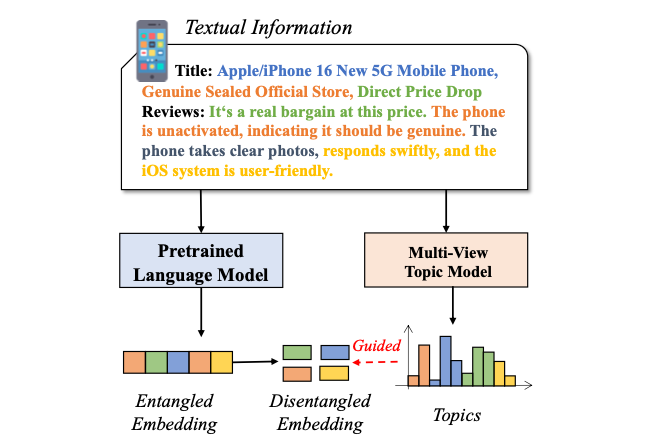
\includegraphics[width=0.9\linewidth]{Figures/Chapter1/figure1.png}
    \caption{Illustration of semantic embedding disentanglement.}
    \label{fig:disentangle}
\end{figure}

Conventional CTR prediction methods typically comprise four main layers: the input layer, embedding layer, interaction layer, and prediction layer. The input layer incorporates a variety of features, including user attributes (e.g., gender, age, occupation, behavior sequences), item characteristics (e.g., category, brand), and contextual information (e.g., interaction location, time). These features are initially processed through the embedding layer to obtain feature embeddings. Subsequently, feature interaction layers, such as Factorization Machines, EulerNet, or KAN, conduct interactions on the feature embeddings. The resulting interacted features are then fed into the prediction layer to estimate the final click probability.

Traditional CTR models primarily rely on structured categorical and numerical features. However, with the rapid advancement of Pretrained Language Models (PLMs), researchers have begun incorporating textual information to enrich semantic understanding and improve prediction accuracy. For instance, CTRL collects textual descriptions of features and encodes them using PLMs to derive semantic embeddings. It employs a contrastive learning strategy to align collaborative signals with these semantic embeddings. Despite the effectiveness of PLMs in extracting semantic features, existing methods typically encode all textual information into a single dense embedding. As illustrated in Figure~\ref{fig:disentangle}, since textual descriptions inherently contain multiple aspects—such as brand, price, quality, and user sentiment—compressing them into a single representation leads to an entangled embedding. This entanglement hinders fine-grained feature interactions, limiting the model’s ability to distinguish between different aspects of user preferences.

Addressing this issue presents two major challenges: 
(1) How can we effectively disentangle and extract meaningful knowledge from textual information? Text descriptions contain rich but interwoven semantic aspects, making it challenging to separate distinct information (e.g., product features, user sentiment, and brand identity) and filter out noise. 
(2) How can we effectively integrate multi-faceted knowledge into the CTR prediction task to extract useful information? Not all extracted textual information is relevant to user decision-making, so aligning it with CTR prediction is crucial for performance improvement.

To address these challenges, we propose \textbf{Multi-faceted Semantic Disentanglement for CTR prediction (MSD-CTR)}. MSD-CTR consists of two components: 
\begin{itemize}
    \item \textbf{Disentangled Semantic Topic Model (DSTopic)} employs a disentangled generative process to capture different aspects of documents using a Disentangled Semantic VAE (DSVAE) and a vocabulary clustering module.
    \item \textbf{Topic Guided Disentangled Representation Learning (TopicDRL)} incorporates the multi-faceted knowledge into CTR prediction, introducing an individual-level alignment loss and an intra-view contrastive loss to guide semantic embedding learning.
\end{itemize}

To evaluate the performance of MSD-CTR, we conduct extensive experiments on four real-world datasets and implement our model based on two foundational CTR methods. The results demonstrate that MSD-CTR outperforms existing CTR models. Additionally, we perform ablation studies and qualitative analyses to validate the effectiveness of the proposed components.

\textbf{Our contributions can be summarized as follows:}
\begin{enumerate}
    \item We investigate text-enhanced CTR methods and analyze the issue of entangled semantic embeddings.
    \item We propose MSD-CTR, a novel framework that disentangles and incorporates multi-faceted knowledge from textual information via DSTopic and TopicDRL modules.
    \item We conduct extensive experiments demonstrating the superior performance of MSD-CTR and validate the contributions of its individual components.
\end{enumerate}


